%  astrochem.tex - Astrochem documentation manual
%
%  Copyright (c) 2006-2012 Sebastien Maret
%
%  This file is part of Astrochem.
%
%  Astrochem is free software: you can redistribute it and/or modify
%  it under the terms of the GNU General Public License as published
%  by the Free Software Foundation, either version 3 of the License,
%  or (at your option) any later version.
%
%  Astrochem is distributed in the hope that it will be useful, but
%  WITHOUT ANY WARRANTY; without even the implied warranty of
%  MERCHANTABILITY or FITNESS FOR A PARTICULAR PURPOSE.  See the GNU
%  General Public License for more details.
%
%  You should have received a copy of the GNU General Public License
%  along with Astrochem.  If not, see <http://www.gnu.org/licenses/>.

\documentclass[a4paper,12pt]{article}

\usepackage{url,graphicx,fancyvrb}
\usepackage[hmargin=2.5cm,vmargin=2.5cm]{geometry}
\usepackage{verbatim} 
\usepackage{natbib}

\newcommand{\aap}{A\&A}
\newcommand{\apj}{ApJ}
\newcommand{\apjs}{ApJS}
\newcommand{\mnras}{MNRAS}
\newcommand{\bain}{Bull.~Astron.~Inst.~Netherlands}

\newcommand{\version}{0.4}
\newcommand{\updated}{June 3, 2011}
\newcommand{\bugreport}{\url{sebastien.maret@obs.ujf-grenoble.fr}}

\newcommand{\conc}[1]{n(\mathrm{#1})}

\begin{document}

\VerbatimFootnotes

\thispagestyle{empty}
\vspace*{5cm}

\noindent
{\huge \textbf{Astrochem}}

\vskip4pt \hrule height 4pt width \hsize

\begin{flushright}
  \noindent
  { \small
    Documentation Manual\\
    For Astrochem version \version\\
    \updated
  }
\end{flushright}

\noindent
{\large \textbf{S\'ebastien Maret}}\\
{\small Institut de Plan\'etologie et d'Astrophysique de Grenoble\\}

\newpage
\vspace*{20cm}

{\small
  \noindent This manual documents Astrochem, a code to compute the
  abundance of chemical species in the interstellar medium. It
  corresponds to Astrochem version \version.
  Please report any errors in this manual to \bugreport.
  \\ \\ \noindent Copyright \copyright \, 2006-2012 S\'ebastien
  Maret
}

\section{What is Astrochem?}
\label{sec:what-astrochem}

Astrochem is a code to compute the abundances of chemical species in
the interstellar medium, as function of time. It is designed to study
the chemistry in a variety of astronomical objects, including diffuse
clouds, dense clouds, photodissociation regions, prestellar cores,
protostars, and protostellar disks\footnote{For the moment, only
  spherical objects with an external radiation field are
  supported.}. Astrochem reads a network of chemical reactions from a
text file, builds a system of kinetic rates equations, and solves it
using a state-of-the-art stiff ordinary differential equations (ODE)
solver. The Jacobian matrix of the system is computed implicitly, so
the resolution of the system is extremely fast: large networks
containing several thousands of reactions are usually solved in a few
seconds. In addition, Astrochem may be run in parallel on multi-cores
and or multi-CPU computers. A variety of gas phase process are
considered, as well as simple gas-grain interactions, such as
freeze-out and desorption via several mechanisms (thermal desorption,
cosmic-ray desorption and photo-desorption). The computed abundances
are written in text files, and can be plotted in different ways with
the tools provided with Astrochem. Chemical reactions and their rates
are written in a format which is meant to be easy to read and to
edit. A tool to convert chemical networks from the
OSU\footnote{\url{http://www.physics.ohio-state.edu/~eric/research.html}}
and KIDA\footnote{\url{http://kida.obs.u-bordeaux1.fr/}} databases
into this format is provided. Astrochem is written in C, and its
source code is distributed under the terms of the GNU General Public
License (GPL).

This manual documents Astrochem. It is organized as follows. The model
is described in section \ref{sec:model}. The various chemical
processes considered in the code and the underlying assumptions are
discussed in this section. Astrochem usage is described in
section~\ref{sec:using-astrochem}. This section is written as a
tutorial: the different steps needed to computed abundances with
Astrochem for a simple case are described. Section
\ref{sec:input-source-files} gives a comprehensive description of
Astrochem input and source model files, while section
\ref{sec:chemical-networks} presents the file format used for chemical
networks in Astrochem, as well as the different networks that are
provided with the code. Section~\ref{sec:runn-astr-parall} explains
how to run Astrochem in parallel. Finally,
Appendix~\ref{sec:astrochem-authors} gives a list of Astrochem
authors, and Appendix~\ref{sec:contr-astr} explains how you can
contribute to the project.

\section{The model}
\label{sec:model}

Abundances in the interstellar medium are usually described by a
system of kinetic equations. For example, let us consider the
HCO$^{+}$ ion. In the dense interstellar medium, this ion is mainly
formed through the reaction:

\begin{equation}
  \mathrm{H_{3}^{+} + CO \rightarrow HCO^{+} + H_{2}}
  \label{eq:hcop-formation}
\end{equation}

\noindent
with a rate $k_{1}$ (in cm$^{3}$~s$^{-1}$ units). HCO$^{+}$ it is
destroyed principally through the following reaction:

\begin{equation}
  \mathrm{HCO^{+} + e^{-} \rightarrow H + CO}
  \label{eq:hcop-destruction}
\end{equation}

\noindent
with a rate constant $k_{2}$. If we neglect other formation and
destruction channels, the derivative of the HCO$^{+}$ density --
i.e. the number of HCO$^{+}$ per volume unit that we note
$\conc{HCO^{+}}$ in the following -- writes as:

\begin{equation}
  \frac{d\conc{HCO^{+}}}{dt} = k_{1} \, \conc{H_{3}^{+}} \, \conc{CO}
  - k_{2} \, \conc{HCO^{+}} \, \conc{e^{-}}
\end{equation}

Similar kinetic equations can be written for all species; therefore to
compute the abundances as a function of time, one need to solve a
system of $n_\mathrm{s}$ equations for a set of initial conditions,
with $n_\mathrm{s}$ the number of species in the chemical
network. These are ordinary differential equations (ODE), that may be
solved by different techniques (Euler method, Runge-Kutta method,
etc.). One difficulty is that the ODE system is usually \emph{stiff},
because of the different timescales considered in the code; for
example, neutral-neutral reactions are typically several orders of
magnitude slower than a ion-neutral reactions. Another characteristic
of the system is that it is \emph{sparse}; many species do not react
together, resulting in a large number of zeros in the Jacobian matrix
of the system\footnote{The Jacobian matrix is a $n_\mathrm{s}^2$
  elements square matrix, whose elements are defined as
  \begin{equation}
     J_{i,j} = \frac{\partial
       \dot\conc{x_{i}}}{\partial \conc{x_{i}}}
   \end{equation}
   \noindent
   with:
   \begin{equation}
     \dot\conc{x_{i}} = \frac{\mathrm{d} \conc{x_{i}}}{\mathrm{d}t}
   \end{equation}}.

 Astrochem reads a set of reactions from a text file (see section~
 \ref{sec:chemical-networks} for a description a chemical network
 files), build-up the system of kinetic equation and solve them using
 the CVODE solver \citep{Cohen96} from the SUNDIALS library
 \citep{Hindmarsh05}. CVODE uses the Backward Differentiation formula
 (BDF method) with a variable step-size, which is suitable for stiff
 systems. The resulting system of linear equations is solved using the
 Newton iteration. The Jacobian matrix of the system is computed
 explicitly to speed-up the computations. In addition, Astrochem may
 be run in parallel on multi core/CPU computers (see
 \S~\ref{sec:runn-astr-parall}). Astrochem includes a number of
 gas-phase chemical processes as well as gas-grain interactions that
 we describe in the following.

\subsection{Gas-phase processes}
\label{sec:gas-phase-processes}
 
\subsubsection{Gas-phase reactions}
\label{sec:gas-phase-reactions}

Most gas-phase reactions have rates that can be described by an
Ahrrenus law:

\begin{equation}
  k = \alpha  \left( \frac{T}{300} \right)^\beta  \mathrm{exp} \left(
    -\frac{\gamma}{T} \right)
  \label{eq:arrhenius}
\end{equation}

\noindent
where $T$ is the gas temperature, and $\alpha$, $\beta$ and $\gamma$
are the rate constants. Usually $\gamma$ corresponds to the energy
barrier of the reaction, expressed in Kelvins. It is generally equal
to zero for ion-neutral reactions, and equal or greater than zero for
neutral-neutral reactions. The units of $k$ depends on the order of
the reaction: for a two body reaction, which is of the second order,
these are cm~$^{3}$~s$^{-1}$.

Astrochem reads the $\alpha$, $\beta$ and $\gamma$ constants from the
chemical network file (see section~\ref{sec:network-file-format} for a
description of the network file format). The formation rate of each
products of a given reaction is then computed by multiplying the
densities of the reactants by $k$. Similarly the destruction rate of
each reactant is computed by multiplying the densities of the
reactants by $k$. Reactions in Astrochem may have up to three
reactants, and four products.

\subsubsection{Cosmic-ray ionization}
\label{sec:cosm-ray-ioniz}

Cosmic-ray particles can ionize molecules and atoms. This may happen
in a direct or indirect fashion. In the first case, the molecule (in
general H$_{2}$) is ionized by a direct interaction with the
cosmic-ray particle. In the second case, the particle first ionizes
H$_{2}$, forming H$_{2}^{+}$ and an electron. The electron then
recombines with H$_{2}^{+}$ and emit a UV photon. This
\emph{secondary} UV photon may then ionize other molecules or
atoms. Astrochem assumes that the rate for these (either direct of
indirect) cosmic-ray ionization reactions scale with the H$_{2}$
ionization rate $\zeta$, such as:

\begin{equation}
  k = \alpha  \, \zeta
  \label{eq:cosmic-ray-ionization}
\end{equation}

\noindent
The value of $\zeta$ is read from the input file (see
section~\ref{sec:input-file}). Typical values are comprised between
10$^{-17}$ and 10$^{-15}$~s$^{-1}$. Note that in this case the units
of $k$ are s$^{-1}$ because cosmic-ray ionization reactions are of the
first order.

\subsubsection{Photo-ionization and photo-dissociation}
\label{sec:photo-ioniz-photo}

UV photons from nearby stars may also dissociate and ionize molecules
and atoms. For sources with a plane-parallel or spherical symmetry,
the ionization or dissociation rate may be written as:

\begin{equation}
  k = \alpha \, \mathrm{exp} \left( -\gamma A_{v} \right) \, \chi
  \label{eq:photo-ionization}
\end{equation}

\noindent
where $A_{v}$ is the visual extinction in magnitude, and $\chi$ is the
external UV flux in Habing units \citep{Habing68}. In other words,
$\chi = 1$ corresponds to a ``standard'' interstellar radiation field
(ISRF).

This formulation implicitly assumes that the external radiation field
has the same spectral shape than the the ISRF. In addition the
\emph{self-shielding} of species that dissociate through a line
process \citep[e.g. CO;][]{vanDishoeck86} is neglected.

\subsection{Gas-grain interactions}
\label{sec:gas-grain-inter}

\subsubsection{H$_{2}$ formation on grains}
\label{sec:h_2-formation-grains}

In the interstellar medium H$_{2}$ is mainly formed on dust grains
\citep{Hollenbach71}. The process is complex and involves the
absorption of an H atom in a grain site, the tunneling of the H atom
from one site to the other, and the reaction with another H to form
H$_{2}$. The energy released during the reactions causes the
evaporation of the H$_{2}$ molecule, which returns to the gas
phase. Astrochem uses a simple treatment of this process.  We assume
that each H atom that strikes a grain forms H$_{2}$ with a given
efficiency. Under this assumption, the formation rate of H$_{2}$ on
the grains is given by:

\begin{equation}
  \frac{\mathrm{d} \conc{H_{2}}}{\mathrm{d} t} = k \, \conc{H}
  \label{eq:h2-formation-rate}
\end{equation}

\noindent
with:
\begin{equation}
  k = \alpha  \left( \frac{T}{300} \right)^\beta
  \label{eq:h2-formation-rate-coeff}
\end{equation}

The value of $k$ may be estimated by assuming that the efficiency of
the process is close to 1 (i.e. that each atom H that strikes a grain
forms an H$_{2}$ molecule). The rate coefficient is then simply $1/2$
of the collision rate between H atoms and grains. For 0.1~$\mu m$
olivine grains and gas-to-dust mass ratio of 100, we obtain a value of
$\sim 10^{-17}$~s$^{-1}$ at 10~K. This is close to the value of $5
\times 10^{-17}$~s$^{-1}$ determined observationally by
\citet{Jura74}. However, because of the numerous uncertainties
associated with the formation of H$_{2}$, in Astrochem the rate is not
computed in this fashion. Instead we use the $\alpha$ and $\beta$
values from the network file, and compute it with
Eq.(\ref{eq:h2-formation-rate-coeff}).

It is important to note that although the formation of H$_{2}$ is a
two body reaction -- if we forget about the grain that only works as a
catalyst -- this reaction has a first order kinetics: the formation
rate of H$_{2}$ depends on $\conc{H}$ and not on
$\conc{H}^{2}$. Because of this, the reaction has its own type number,
0 (see Table~\ref{tab:react-type-numb}). At present the formation of
H$_{2}$ on grains is the only grain surface reaction that is
considered in Astrochem.

\subsubsection{Electron attachment and ion recombination on grains}
\label{sec:electr-attachm-ion}

Electron may hit grains and charge them. Ions may then recombine on
charged grains. For example, let us consider the following reactions:

\begin{equation}
  \mathrm{grain} + e^{-} \rightarrow \mathrm{grain}^{-}
\end{equation}

\begin{equation}
  \mathrm{C^{+}} + \mathrm{grain}^{-} \rightarrow \mathrm{C} + \mathrm{grain}
\end{equation}
 
The formation rate of charged grains writes as:

\begin{equation}
  \frac{d \conc{grain^{-}}}{\mathrm{d}t} = k_{1} \, \conc{grain} \, \conc{e^{-}}
\end{equation}

\noindent
while the recombination rate of $\mathrm{C^{+}}$ is:

\begin{equation}
  \frac{d \conc{C^{+}}}{\mathrm{d}t} = - k_{2} \, \conc{grain^{-}} \, \conc{C^{+}}
\end{equation}

Both $k_{1}$ and $k_{2}$ are computed from the following expression:

\begin{equation}
  k = \alpha \left( \frac{T}{300} \right)^\beta \, \frac{n_\mathrm{H}}{n_\mathrm{d}}
  \label{eq:grain-attach-neutralization}
\end{equation}

\noindent
where $n_\mathrm{H}$ is the total hydrogen nuclei density\footnote{In
  other words:

  \begin{equation}
    n_\mathrm{H} = \conc{H} + 2 \, \conc{H_{2}} + 3 \,
    \conc{H_{3}^{+}} + ...
  \end{equation}
  
  Abundances computed by Astrochem are always with respect to
  $n_\mathrm{H}$.}  and $n_\mathrm{d}$ is the total (neutral +
charged) grain density. The $\frac{n_\mathrm{H}}{n_\mathrm{d}}$ ratio
is assumed to be $7.57 \times 10^{11}$, a value adequate for olivine
grains of 0.1~$\mu$m and a gas-to-dust mass ratio of 100\footnote{The
  formulation for this process, and in particular normalization of the
  rate by the $\frac{n_\mathrm{H}}{n_\mathrm{d}}$ may sound a bit
  awkward. In fact, Astrochem treats the electron attachment and
  recombination in this fashion essentially for compatibility with the
  OSU database. This may change in future releases of the code.}

$k_{1}$ may be estimated by assuming that each electron that hits a
grain will attach to it. For 0.1~$\mu m$ olivine grains and
gas-to-dust mass ratio of 100, we obtain a value of $\sim
10^{-3}$~cm$^{-3}$~s$^{-1}$ at 10~K. This process is extremely fast
because electron have large thermal velocities (thanks to their small
masses). In practice, in simulations free electrons almost immediately
stick on the grains, so that grains become negatively charged very
rapidly.

\subsubsection{Depletion}
\label{sec:depletion}

Molecules may accrete on dust grains and freeze-out (a process often
called depletion). The formation rate of e.g. ices CO on the grains
through this process is given by:

\begin{equation}
  \frac{\mathrm{d}\conc{CO_{ice}}}{\mathrm{d}t} = k \, \conc{CO}
\end{equation}

\noindent
with:
\begin{equation}
  k = S \, \pi r_{d}^2 \, v_{th} \, n_\mathrm{d}
  \label{eq:freeze-out}
\end{equation}

\noindent
and:
\begin{equation}
  v_{th} = \left( \frac{8 k_{B} T_{d}}{\pi m} \right)^{1/2}
  \label{eq:thermal-veloc}
\end{equation}

\noindent
Here $S$ is a sticking probability (comprised between 0 and 1),
$r_{d}$ is the grain radius, $v_{th}$ is the thermal velocity, $n_{d}$
is the total grain density (neutral + charged) and $m$ is the mass of
the accreting species \citep{Bergin95}.

Because no grain destruction or formation mechanisms are considered in
Astrochem, $n_{d}$ does not varies with time. It is therefore computed
from the initial abundances of neutral and charged grains given in the
input file (see section~\ref{sec:initial-abundances}). The grain size
$r_{d}$ is also read from this file. Both $S$ and $m$ are read from
the network file.

\subsubsection{Thermal desorption}
\label{sec:thermal-desorption}

Once frozen on the dust grains, molecules may evaporate through
thermal or non-thermal processes. The formation rate of gaseous CO by
CO ices thermal evaporation is:

\begin{equation}
  \frac{\mathrm{d}\conc{CO}}{\mathrm{d}t} = k \, \conc{CO_{ice}}
\end{equation}

\noindent
where $k$ is given by the Polanyi-Wigner equation:

\begin{equation}
  k = \nu_{0} \, \mathrm{exp} \left( - \frac{E_{B}}{T_{d}} \right)
  \label{eq:thermal-desorption}
\end{equation}

\noindent
with:

\begin{equation}
  \nu_{0} = \left( \frac{2 N_{S} E_{B}}{\pi^2 m} \right)^{1/2}
  \label{eq:vibration-freq}
\end{equation}

\noindent
Here $\nu_{0}$ is the characteristic vibrational frequency of the
desorbing species, $E_{B}$ is the binding energy of the desorbing
species on the grain surface expressed in Kelvins, $T_{d}$ is the
grain temperature and $N_{S}$ is the number of sites per unit surface
assumed to be $3 \times 10^{15}$~cm$^{-2}$ \citep{Hasegawa92}. The
values of $E_{b}$ and $m$ are both read from the network file.

\subsubsection{Cosmic-ray desorption}
\label{sec:cosm-ray-desorpt}

As mentioned above, ices may also evaporate by non-thermal
processes. For example, cosmic-rays may desorb molecules from grains,
either by creating hot-spots on the grain surfaces, or by heating the
whole grains \citep{Leger85}. Because the energy deposited in a grain
varies as $Z^{2}$, cosmic-ray desorption in mainly caused by heavy
cosmic-ray ions, such as Fe. \cite{Leger85} suggested that desorption
by spot-heating dominates over desorption by whole-grain heating for
grains smaller than 2.5 $\mu$m. However, recent molecular dynamics
simulations indicate that for 0.1 $\mu$m grains the whole grain
heating contribution is small \citep{Bringa04}.

Because of the uncertainties on this process, two different treatments
are implemented in Astrochem. First, cosmic-ray desorption rates can
be computed following \citet{Hasegawa93}, who assume that desorption
occurs mostly through whole-grain heating; when impacting grains,
heavy cosmic-ray ions are assumed to impulsively heat the grains to a
peak temperature of 70~K, at which most of the desorption occurs. The
rate is then similar to that of thermal desorption:

\begin{equation}
  k = f \, \nu_{0} \, \mathrm{exp} \left( -\frac{E_{B}}{70} \right)
  \label{eq:cosmic-ray-desorption}
\end{equation}

\noindent
where $f$ is the fraction of the time spent by a grain in the vicinity
of 70~K between two cosmic-ray heating events, assumed to be $3.16
\times 10^{-19}$ \citep{Hasegawa93}.

Alternatively, the cosmic-ray desorption rate of any specie can be
given explicitly in the network file. This allows for the use of the
cosmic-ray desorption rates that have been computed and/or measured
for some species \citep[e.g. H$_{2}$O and CO;][]{Bringa04}. The user
can specify in the network file which treatment to use for each species
(see Table.~\ref{tab:rate-const-meaning}).  Note that no scaling of
$k$ with the cosmic ray ionization rate is performed.

\subsubsection{Photo-desorption}
\label{sec:photo-desorption}

Photo-desorption (i.e. desorption by UV photons) is another
non-thermal desorption process. UV photons can originate in the ISRF,
or in the ionization of H$_{2}$ by cosmic-rays followed by
recombination (secondary UV photons). At present only photo-desorption
from ISRF UV photons is implemented in Astrochem.

The photo-desorption rate of CO is for example
\citep{Oberg09a,Oberg09b}:

\begin{equation}
  \frac{\mathrm{d} \conc{CO}}{\mathrm{d} t} = k
  \label{eq:photo-desorption-rate}
\end{equation}  

with:
\begin{equation}
  k = \chi \, G_{0} \, \mathrm{exp} \left( -2 A_{v} \right)
  \, \pi r_{d}^{2} \, n_{d} \, Y_\mathrm{PD}
  \label{eq:photo-desorption}
\end{equation}

\noindent
Here $G_{0}$ is the average UV ISRF \citep[assumed to be
10$^{8}$~photons~cm$^{-2}$~s$^{-1}$;][]{Habing68}, and $Y_\mathrm{PD}$
is the photo-desorption yield, i.e. the number of molecules ejected
per incident photon. The latter is given by:

\begin{equation}
  Y_\mathrm{PD} = Y_{0} \left[ 1 - \mathrm{exp} \left( -x / l \right) \right]
  \label{eq:photo-desorption-yield}
\end{equation}

\noindent
where $x$ is the ice thickness of the considered species expressed in
monolayers (ML), $l$ is the diffusion length in ML, and $Y_{0}$ is the
photo-desorption yield for thick ices (i.e. $x \gg l$). Typical values
for $Y_{0}$ and $l$ are $10^{-3}$ molecules~photon$^{-1}$ and 2~ML,
respectively\footnote{For some species, $Y_{0}$ depends weakly on the
  dust temperature \citep{Oberg09a}. This effect is not implemented in
  Astrochem.}. The density of e.g. CO ices is given by:

\begin{equation}
  x = \frac{\conc{CO_{ice}}}{N_{s} \, \pi r_{d}^2 \, n_{d}}
  \label{eq:ice-thickness}
\end{equation}

\noindent
It is interesting to note that for thick ices, photo-desorption is
zeroth order process: the desorption rate does not depends on the
amount of e.g. CO ices on the grains. This because UV photons can
penetrate only the first ices monolayers; the bulk of ice is not
affected. On the other hand, for thin ices (i.e. $x \ll l$) the
desorption rate become linearly proportional to the ice thickness, and
therefore on the ice abundance. Consequently for thin ices,
photo-desorption is a first order process.

Astrochem follows the ice thickness of each species as a function of
time. The desorption rate is then computed from the above equations,
using the values of $\chi$, $r_{d}^2$ and $n_{d}$ from the input file,
the $A_{v}$ from the source file, and the $Y_{0}$ and $l$ from the
network file.

\section{Using Astrochem}
\label{sec:using-astrochem}

In this section we present a simple example of Astrochem usage.  We
propose to use Astrochem to study the formation of the HCO$^{+}$ ion
in a dense interstellar cloud. We suppose that the cloud is isodense
and isothermal, and that it is shielded from the ISRF, so that
photo-processes can be ignored. For a sake of simplicity, we also
neglect the freeze-out of  molecules on dust grains. In the following,
we describe the various steps needed to solve this problem.

\subsection{Describing the problem}
\label{sec:describing-problem}

In order to describe our problem, we first need create an input file
that contains the various parameters the code. This file has several
sections, that set the physical parameters (e.g. the cosmic ionization
rate), the solver parameters (e.g. the initial and final time in the
computation), the initial abundances, and which species we want in
output. Some of these parameters are optional; if they are not
specified in the input file, Astrochem will use a default value that
should be suitable for most problems. Here is a what the input file
for our example problem looks like (for a comprehensive description of
the parameters in input files and their default value, see
section~\ref{sec:input-file}):

\begin{verbatim}
[files]
source = source.mdl
chem = osu2009.chm
# Physical paramaters
[phys]
chi = 1.0
cosmic = 1.3e-17
# Solver parameters
[solver]
ti = 1e-6
tf = 1e7
# Initial abundances
[abundances]
H2      = 0.5
He      = 0.14
N       = 2.14e-5
O       = 1.76e-4
C(+)    = 7.30e-5
S(+)    = 8.00e-8
Si(+)   = 8.00e-9
Fe(+)   = 3.00e-9
Na(+)   = 2.00e-9
Mg(+)   = 7.00e-9
P(+)    = 2.00e-10
Cl(+)   = 1.00e-9
F       = 6.68e-9
e(-)    = 7.31012e-5
# Output
[output]
abundances = H3(+),e(-),CO,HCO(+)
trace_routes = 1
\end{verbatim}

The various sections of the file are indicated by keywords within
brackets. Lines starting with \verb=#= are comments. The first section
(\verb=[files]=) indicates the name of the file describing our source
(\verb=source=), and the chemical network to use (\verb=chem=). The
following section (\verb=[phys]=) sets the physical parameters of the
source. Here we set the interstellar radiation field (\verb=chi=) to
1.0 (in Habing units), and the cosmic ionization rate (\verb=cosmic=)
to $1.3 \times 10^{-17} s^{-1}$. The solver parameters are set in
following section (\verb=[solver]=). \verb=ti= and \verb=tf= are the
initial and final time for the calculation respectively. Both are
expressed in years. The \verb=[abundance]= section sets the initial
abundances; abundances that are not specified are set to zero. The
last section (\verb=[output]=) sets parameters relative to the output
of the code. \verb=abundances= set the name of the species for which
we want to create output files containing the abundances as a function
of time. \verb=trace_route= is an optional parameter that allow to
trace the various formation and destruction routes of these species.

In addition to the input file, we need to provide a file describing
our source. The file corresponding to our problem looks like this (for
more information on source model files, see
section~\ref{sec:source-file}):

\begin{verbatim}
# Source model file example
# shell number, Av [mag], nH [cm^-3], Tgas [K], Tdust [K]
#
0	20.0	1e+04	10.0	10.0
\end{verbatim}

As for the input file, lines that starts with a \verb=#= are
comments. The file contains one line for each \emph{shell} of our
source. In this simple example, our source is isodense and isothermal,
and therefore there is only one shell in the our source file. A more
realistic source with a temperature and density gradient would be
sampled in more shells.

Each line corresponding to a shell has five columns. The first column
is the index of the shell, the second one is the visual extinction
$A_{v}$ (in magnitudes), the third one is the number density (in
cm$^{-3}$). and the fourth and the fifth are the gas and dust
temperature respectively (in Kelvins).  Note that we have adopted a
large visual extinction (20 mag.), that is suitable for dense clouds
shielded from the ISRF.

\subsection{Running Astrochem}
\label{sec:running-astrochem}

Astrochem is run from the command line, and takes the name of the
input file as an argument:

\begin{verbatim}
% astrochem input.ini
Reading input from input.ini.
Reading source model from source.mdl.
Reading reactions network from osu2009.chm... done.
Found 6046 reactions involving 468 species.
Computing abundances in shell 0...
Done with shell 0.
Writing abundances in output files... done.
Writing formation/destruction in output files... done.
%
\end{verbatim}

Astrochem produces two types of files: the \verb=.abun= files that
contain the abundance of a given species as a function of time and --
if the \verb=trace_route= parameter is set to 1 -- the \verb=.rout=
files that contain the main formation and destruction routes of a
given specie.

With the input file above, Astrochem creates the following abundances
files: \verb=H3(+).abun=, \verb=CO.abun=, \verb=e.abun= and
\verb=HCO(+).abun=. Note that each file contains the abundance of a
single specie. The first lines of the \verb=HCO(+).abun= file looks
like this:

\begin{verbatim}
# HCO(+) abundance computed by astrochem
# time [yr] / shell number
#
                 0
1.00e-06  0.00e+00
2.63e-06  0.00e+00
6.90e-06  0.00e+00
1.81e-05  6.30e-20
4.76e-05  4.28e-19
1.25e-04  2.91e-18
3.28e-04  1.97e-17
8.62e-04  1.29e-16
2.26e-03  7.74e-16
5.95e-03  3.84e-15
1.56e-02  1.33e-14
4.10e-02  2.82e-14
1.08e-01  3.57e-14
2.83e-01  4.02e-14
7.43e-01  5.04e-14
1.95e+00  7.00e-14
5.12e+00  9.52e-14
(...)
\end{verbatim}

\noindent
The first three lines are comments. The third one lists the shell
indexes. The following lines gives the abundances as a function of
time for each shell; the first column indicates the time in year, and
the following ones the abundances, with respect to H nuclei, in each
shell. In our simple example, there is only one shell, so the file has
only two columns, one for the time, and one for the shell number.

\subsection{Plotting abundances}
\label{sec:plotting-abundances}

Astrochem comes with a program that make plots of the abundances
computed by Astrochem. The program, named Plabun, allows to plot the
abundances of one or several species as of function of time in a given
shell, or as a function of position at a given time. For example, the
following command plots the CO, H$_{3}^{+}$, e$^{-}$ and HCO$^{+}$
abundances as a function of time:

\begin{verbatim}
% plabun --xrange=1,1e7 --yrange=1e-12,1e-4 time CO.abun H3\(+\).abun
e.abun HCO\(+\).abun
\end{verbatim}

In the example above, we have set the x-axis range from 1 to 10$^{7}$
yr and y-axis range from $10^{-12}$ to $10^{-4}$ with the
\verb=--xrange= and \verb=--yrange= options, respectively. The
\verb=time= commands tells Plabun to plot abundances as function of
time in the first (and unique in our case) shell. Note that
parenthesis in files names such as \verb=H3(+).abun= needs to be
preceded by an anti-slash (\verb=\=) because they have a special
meaning for Unix shells. The command above produces the plot shown on
Fig.~\ref{fig:example-abundances}. Plabun has a number or other
commands and options; see \verb=man plabun= for a complete list.

\begin{figure}
  \begin{center}
    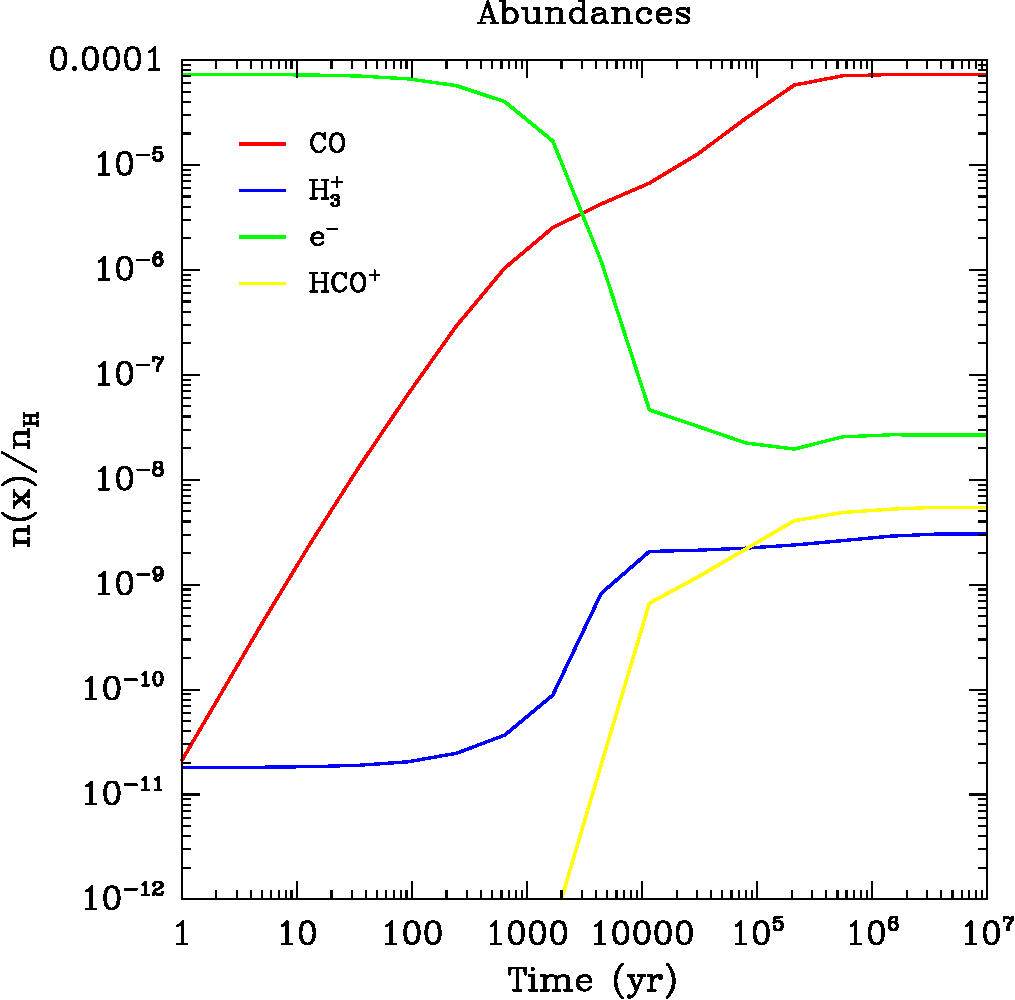
\includegraphics[height=10cm]{fig1.pdf}
  \end{center}
  \caption{Abundances as a function of time for the example problem.}
  \label{fig:example-abundances}
\end{figure}

\subsection{Identifying the main formation and destruction channels of
   a species}
\label{sec:ident-main-form}

It is often useful to identify the main formation and destruction
routes of a given species, for example to check that the rate of these
main reactions have been determined accurately (e.g. from experiments)
or are rather uncertain. This also allows to understand how the
various species of a chemical network are linked together.

As already mentioned, if one turns on the \verb=trace_route= option
in the input file, Astrochem creates some additional files containing
the main formation and destruction routes of the species listed with
\verb=output= option. Of course these routes may change with time;
therefore Astrochem saves the sixteen most important formation routes
as well as the sixteen most important destruction routes at each time
step and position.

Although the \verb=.rout= files are text files, they are -- unlike
the \verb=.abun= files -- not easy to read directly. However a command
allows to plot the main formation and destruction rate of a given
species as a function of time or position\footnote{Plotting the main
  formation/destruction routes as a function of position is not
  implemented yet.}. For example, one can plot the main formation and
destruction routes of HCO$^{+}$ with the following command (see
\verb=man plroute= for a complete list of commands and options):

\begin{verbatim}
% plroute --chmfile=osu2009.chm time HCO\(+\).rout
\end{verbatim}

\begin{figure}
  \begin{center}
    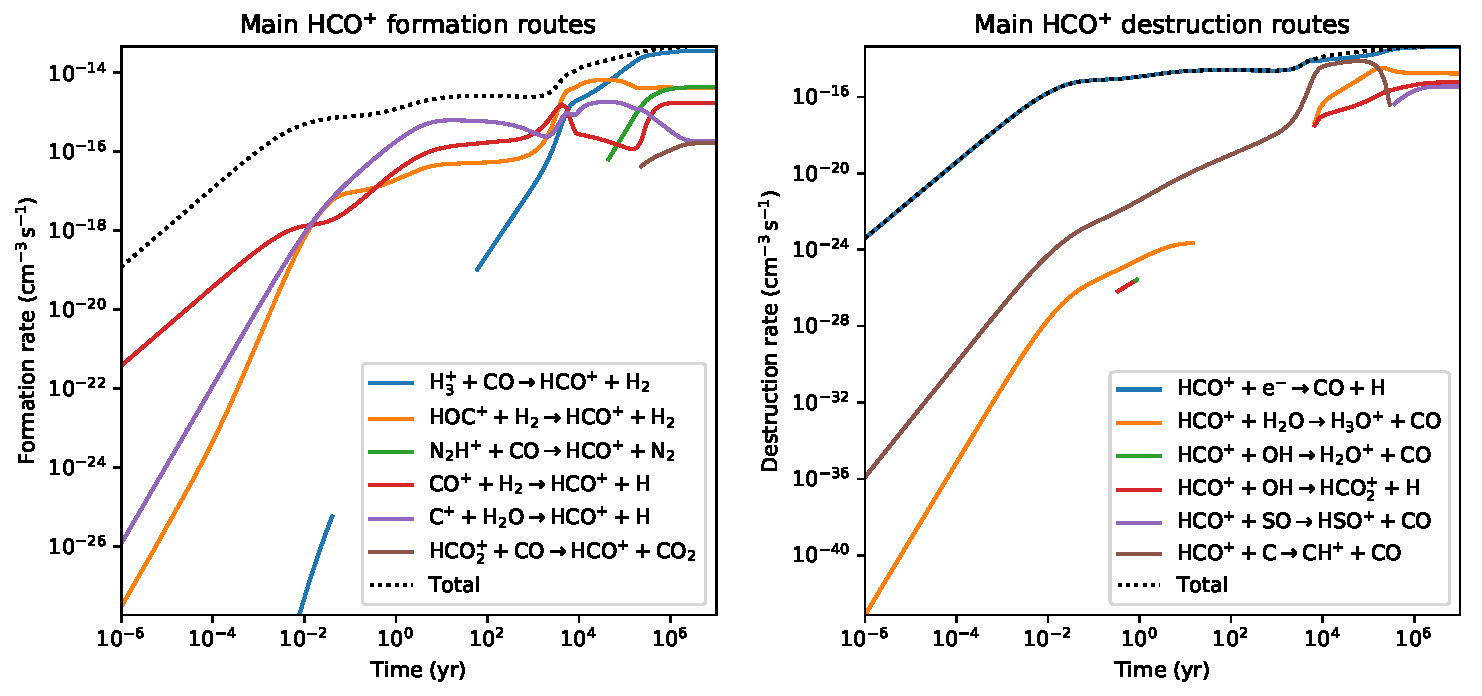
\includegraphics[width=\columnwidth]{fig2.pdf}
  \end{center}
  \caption{Main HCO${+}$ formation and destruction routes as function
    of time for the example problem.}
  \label{fig:example-routes}
\end{figure}

\noindent
which produces the plot shown on Fig.~\ref{fig:example-routes}.

The left panel of the plot shows the formation rate of HCO$^{+}$ (in
cm$^{-3}$~s$^{-1}$) through the six most important formation
channels\footnote{The formation and destruction reactions are ordered
  by the integral of their formation/destruction rate over
  time. i.e. their total contribution to the formation/destruction of
  the species. The \verb=--percent= option allows to display the
  relative contribution, expressed in percent, to the
  formation/destruction of the species.}, together with the total
formation rate. Conversely, the right panel shows the destruction rate
of the same species through the six most important destruction
channels as well as the total destruction rate. The \verb=--chmfile=
option followed by the name of the network used in the computation
makes Plabun to print the reactions explicitly instead of printing
their numbers. On the left panel, we see that for $t > 10^{5}$~yr, the
formation of HCO$^{+}$ is dominated by the reaction of CO with
H$_{3}^{+}$. On the other hand, at any time in the simulation the
destruction of HCO$^{+}$ is dominated by the dissociative
recombination with electrons.

Note that because Astrochem only keeps tracks of the sixteen most
important formation or destruction routes at any time, some gaps may
appear in the plot. This can been seen for the reaction in red on the
left panel of the plot for times between roughly 0.1 and 10 years. In
this time range this reaction is not one the sixteen most important
formation reaction, so Astrochem does not keep track of it in this
time range.

\section{Input and source files}
\label{sec:input-source-files}

\subsection{Input file}
\label{sec:input-file}

As mentioned already, the various parameters of Astrochem are read
from an input file. Although this is not mandatory, the file usually
has the \verb=.ini= file extension. The file has several sections that
are delimited by a keyword within brackets (e.g. \verb=[files]=). Each
section has a number of parameters that we describe in the following.

\subsubsection{Files}
\label{sec:files}

This section of the file starts with the \verb=[files]= keyword, and
specifies which file Astrochem should use for the source description
(\verb=.mdl= file) and chemical network (\verb=.chm= file). The
parameters allowed in this section are:

\begin{itemize}

\item \verb=source=: The name of the file describing the source.

\item \verb=network=: The name of the chemical network file. First
  Astrochem searches for this file in the current directory. If not
  found, it then searches for the file in Astrochem data installation
  directory (\verb=/usr/local/share/astrochem= by default).

\end{itemize}

\subsubsection{Physical parameters}
\label{sec:physical-parameters}

This section of the file starts with the \verb=[phys]= keyword and
specifies the physical parameters of the problem. These parameters
are:

\begin{itemize}

\item \verb=chi=: The external radiation field, expressed in
  \citet{Habing68} units. This corresponds to $\chi$ in
  Eq.~(\ref{eq:photo-ionization}) and Eq.~(\ref{eq:photo-desorption}).

\item \verb=cosmic=: The cosmic ray ionization rate of molecular
  hydrogen expressed in s$^{-1}$. The default value is $1.3 \times
  10^{-17}$. This corresponds to $\zeta$ in
  Eq.~(\ref{eq:cosmic-ray-ionization}).

\item \verb=grain_size=: The grain radius in microns. The default
  value is 0.1. This corresponds to $r_{d}$ in
  Eq.~(\ref{eq:freeze-out}) and Eq.~(\ref{eq:photo-desorption}).

\end{itemize}

\subsubsection{Solver parameters}
\label{sec:solver-parameters}

This section of the file starts with the \verb=[solver]= and specifies
the ODE solver parameters. These parameters are:

\begin{itemize}

\item \verb=ti=: The initial time for the computation, expressed in
  years. The default value is $10^{-6}$.

\item \verb=tf=: The final time for the computation, expressed in
  years. The default value is $10^{7}$.

\item \verb=abs_err=: The solver absolute error (or tolerance) on the
  computed abundances. The default value is $10^{-20}$.

\item \verb=rel_err=: The solver relative error on the computed
  abundances. The default value is $10^{-6}$.

\end{itemize}

A note on tolerances: Astrochem adjusts the internal time step so that
the relative error on any abundance is always lower that
\verb=rel_err=, unless the given abundance is lower that
\verb=abs_err=. Because errors on the abundances at each time step may
add-up, we recommend to chose these errors quite conservatively. The
default values should be suitable for most problems.

\subsubsection{Initial abundances}
\label{sec:initial-abundances}

This section specifies the initial abundances in the computation. Each
line should contain a specie name followed by a equal sign and the
initial abundance with respect to H nuclei. The initial abundances of
species that are not listed in this section are assumed to be
zero. Note that grains must be written as \verb=grain=,
\verb=grain(-)= or \verb=grain(+)= so that the total grain density
$n_{d}$ is computed correctly (see section~\ref{sec:depletion}).

\subsubsection{Output}
\label{sec:output}

This section specifies what file Astrochem should create at the end of
the computation. These parameters are:

\begin{itemize}

\item \verb=output=: The name of the species for which Astrochem
  creates an output file containing the abundance as a function of
  time and position. Species names must be separated by a comma. File
  names are formed with the species name, possibly followed by a
  suffix (see below) and the \verb=.abun= file extension.

\item \verb=suffix=: A suffix to append to the name of the species
  before the file extension (\verb=.abun= or \verb=.reac=) in
  abundance files. This is useful when you want to run Astrochem for a
  number of different input files all located in the same directory;
  this way the results of a given simulation will not be overwritten
  by the results of others. A leading underscore is added to this
  suffix.

\item \verb=time_steps=: The number of time steps in output the
  files\footnote{Output files contain abundances for \verb=time_steps=
    time values that are logarithmically sampled between \verb=ti= and
    \verb=tf=.}. The default value is 32. If plots of abundances
  v.s. time appear somewhat boxy, you may increase this number. Note
  that this parameter only affects the number of time steps in the
  output files. The internal time step size is set by the ODE solver
  in order to reach the specified absolute and relative errors on the
  abundances.

\item \verb=trace_routes=: This parameter is used to toggle the
  computation of the major formation and destruction routes for all
  species listed with the \verb=output= parameter. If
  \verb=trace_route= is set to 1, Astrochem will create a file
  containing the formation/destruction rate and reaction number of the
  16 most important formation/destruction reaction for each specie, as
  a function of time and position (i.e. shell number). As for
  abundance files, file names for formation and destruction routes are
  formed with the species name possibly followed by a suffix (see
  below) and the \verb=.rout= file extension.

\end{itemize}

\subsection{Source file}
\label{sec:source-file}

Astrochem reads the physical parameters (density, temperature) of the
astronomical source in a source file. Although the source may have in
principle any dimension, Astrochem is, for the moment, only designed
to study 1D spherical sources in an external radiation field (such as
a dense cloud or a prestellar core in the ISRF). Future versions will
allow to study 2D sources with axisymmetrical geometries, such as
protoplanetary disks.

In order to construct a source model file, one needs to sample the
astronomical source in a number of spherical shells at different
source radius. What constitutes a good sampling depends on the
source. Often density profiles of astronomical sources are well
described by a power laws, so it is usually a good idea to sample the
source in a number of logarithmically spaced shells. Of course, the
larger number of shells, the longer computational time. However,
Astrochem may be run in parallel on multi-cores computer in order to
reduce computational time (see section~\ref{sec:runn-astr-parall}).

Each line of the file corresponds to a different shell, while each
column corresponds to a different parameter. These parameters are,
from the leftmost to the rightmost columns:

\begin{enumerate}

\item The shell index. This is an integer that is used to identify
  each shell. The first index should be 0. Other indexes in the file
  should be in increasing order. All shells should have a different
  index.

\item The visual extinction in the shell, expressed in magnitudes.

\item The H nuclei density in the shell, expressed in cm$^{-3}$.

\item The gas temperature in the shell, expressed in K.

\item The dust temperature in the shell, expressed in K.

\item The radius corresponding to the shell, expressed in astronomical
  units (AU). This optional parameter is used by Plabun only when
  plotting abundances as a function of the source radius (see
  \verb=man plabun= for more information); Astrochem ignores it.

\end{enumerate}

\noindent
Columns may be separated by any number of white spaces or
tabs. Comments may written in the source file; comment lines must
start with a \verb=#= sign.

\section{Chemical networks}
\label{sec:chemical-networks}

Astrochem reads the chemical reactions and their rate coefficient from
a chemical network file. This file should have \verb=.chm=
extension. Several networks are distributed with Astrochem, but the
user may also write its own network. In the following, we describe the
networks files that are distributed with Astrochem, as well as the
format of these files. Finally, we explain how networks in other
formats can be converted to Astrochem format.

\subsection{Networks provided with Astrochem}
\label{sec:netw-prov-with}

The following networks are provided with Astrochem:

\begin{itemize}

\item \verb=osu2009.chm=: This network file contains the reactions and
  rates from the Ohio State University (OSU) astrochemistry database, that
  is maintained by Eric Herbst. It corresponds to the January 2009
  version of the database. This network contains 6046 reactions and
  468 species, including anions.

\item \verb=osu2008.chm=: This network file contains the September
  2008 version of OSU database.  It includes 4457 reactions and 452
  species (no anions).

\end{itemize}

These networks can be found in the network directory of the source
distribution. When installing Astrochem, these file are copied in the
data installation directory \\(\verb=/usr/local/share/astrochem= by
default). 

\subsection{Network file format}
\label{sec:network-file-format}

Astrochem network file format is meant to be easily read and
edited. Therefore chemical reactions in this files are written as you
would write them on a piece of paper. Here is an example of a
(incomplete) network file:

\begin{verbatim}
# A few reactions extracted from osu2008.chm
H     + H          -> H2                 4.95e-17  5.00e-01  0.00e+00  0    1
H2    + cosmic-ray -> H2(+)  + e(-)      9.30e-01  0.00e+00  0.00e+00  1   39
H3(+) + CO         -> HCO(+) + H2        1.61e-09  0.00e+00  0.00e+00  2 1756
H3(+) + e(-)       -> H      + H    + H  4.36e-08 -5.20e-01  0.00e+00  9 3746
CO    + uv-photon  -> C      + O         3.10e-11  0.00e+00  2.54e+00 13 4297
(...)
\end{verbatim}

As for input and model files, lines that starts with the \verb=#=
character are comments. Each line of the file corresponds to a
different reaction. Lines have two parts: the chemical equation, and a
list of five numbers that correspond to the rate constants, reaction
type and reaction number.

The chemical equation is composed of one, two or three reactants, and
one, two, three or four products. Each reactants and products are
separated by a white space, a \verb=+= sign, and another white
space. To disentangle the \verb=+= sign between reactants from the ones
corresponding to ions, ion charge must be put in parenthesis: for
example, the HCO$^{+}$ ion must be written as \verb=HCO(+)= in the
network file. Reactants and products are separated by a white space,
an arrow (\verb=->=), and another white space.

In general, Astrochem computes the formation rate of each product (or
the destruction rate of each reactant) through a given reaction by
multiplying the reaction rate by the product of the reactants. For
example, for the reaction:

\begin{verbatim}
H3(+) + e(-)       -> H      + H    + H  4.36e-08 -5.20e-01  0.00e+00  9 3746
\end{verbatim}

\noindent
the destruction rate of H$_{3}^{+}$ and e$^{-}$ is computed as:

\begin{equation}
  \frac{d \conc{H_{3}^{+}}}{dt} = \frac{d \conc{e^{-}}}{dt} = - k \,
  \conc{H_{3}^{+}} \, \conc{e^{-}}
\end{equation}

\noindent
while the formation rate of H is computed as:

\begin{equation}
  \frac{d \conc{H}}{dt} = k \, \conc{H_{3}^{+}} \, \conc{e^{-}}
\end{equation}

\noindent
In other words, one body reactions (e.g. cosmic-ray ionization, or UV
ionization) are assumed to have a first order kinetics, two body
reactions are assumed to have a second order kinetics, etc. However,
there are two exceptions to this rule. First the formation of H$_{2}$
on the grains is assumed to be of the first order (see
section~\ref{sec:h_2-formation-grains}). Second, UV photodesorption is
assumed to have a zeroth order kinetics when the ice thickness is
large enough (see \S~ref{sec:photo-desorption}).

Several reactants and products are not \emph{bona fide} chemical
species, but are just meant to make the reading of the network
easier. These \emph{pseudo-species} are \verb=cosmic-ray= (for
cosmic-ray direct or indirect ionization or desorption reactions),
\verb=uv-photon= (for photo-ionization, photo-dissociation and
photo-desorption reactions) and \verb=photon= (for radiative
association reactions). All of these are ignored by Astrochem.

The five numbers following the products are the three rate constants
(that we note $a$, $b$ and $c$ respectively), the reaction type, and
the reaction number. The reaction type is a signed integer that
identifies the kind of the reaction (e.g. ion-molecule, dissociative
recombination, etc.). Table~\label{tab:react-typea-numb} lists the
various reaction types together corresponding type
numbers\footnote{The reaction types adopted in Astrochem follows
  closely that used in the OSU database.}. The reaction number is an
integer that identify each reaction in a unique fashion: every
reaction must have a different number. Reaction numbers must start at
1, but they are not necessarily contiguous. For example you may want
to identify gas-phase reactions by numbers between 1 and 6046, and
gas-grain reactions by numbers starting at 10000.

\begin{table}
  \begin{center}
    \caption{Reaction types and their corresponding type numbers.}
    \begin{tabular}{ll}
      \hline
      \hline
      Type number & Reaction type\\
      \hline
      -1 & Electron attachment and ion recombination on grains\\
      0  & H$_{2}$ formation on grains\\
      1  & Cosmic-ray ionization or cosmic-ray induced photo-reactions\\
      2  & Ion-molecule reactions, Charge exchange reactions\\
      3  & Negative ion - neutral species reactions\\
      4  & Radiative association\\
      5  & Associative ejection\\
      6  & Neutral + Neutral $\rightarrow$ ion + electron\\
      7  & Neutral-Neutral chemical reactions\\
      8  & Neutral-Neutral radiative association\\
      9  & Dissociative recombination\\
      10 & Radiative recombination\\
      11 & Positive ion - Negative ion recombination\\
      12 & Electron attachment\\
      13 & Photo-ionization, Photo-dissociation\\
      20 & Freeze-out on grains\\
      21 & Thermal desorption\\
      22 & Cosmic-ray induced desorption\\
      23 & Photo-desorption\\
      \hline
    \end{tabular}
    \label{tab:react-type-numb}
  \end{center}
\end{table}

Astrochem computes the rate of each reaction from the $a$, $b$ and $c$
rate constants. The physical meaning of these constants depends on the
type of the reaction. Table~\label{tab:rate-const-meaning} gives
physical meaning of these for each reaction type, as well as the
equation that is used to computed the rate. Because reaction rates
generally do not vary with time, Astrochem computes them only once for
each shell. The only exception is the rate of UV photo-desorption
reactions, that depends on the ice thickness; therefore the rate for
these reactions is computed for each solver internal time step.

\begin{table}
    \renewcommand{\footnoterule}{}  
    \begin{center}
      \caption{Physical meaning of the rate constants used chemical
        networks and equation used in the code to compute the reaction
        rate for each reaction type.}
      \begin{tabular}{llccc}
        \hline
        \hline
        Type number & Equation & \multicolumn{3}{c}{Rate constants}\\
        \cline{3-5}
        & & $a$ & $b$ & $c$\\
        \hline
        -1    & Eq.~(\ref{eq:grain-attach-neutralization}) & $\alpha$ & $\beta$\\
        0     & Eq.~(\ref{eq:h2-formation-rate}) & $\alpha$ & $\beta$\\
        1     & Eq.~(\ref{eq:cosmic-ray-ionization}) & $\alpha$ & - & -\\
        2-12  & Eq.~(\ref{eq:arrhenius}) & $\alpha$ & $\beta$ & $\gamma$\\
        13    & Eq.~(\ref{eq:photo-ionization}) & $\alpha$ & - & -\\
        20    & Eq.~(\ref{eq:freeze-out}) & $S$ & $m/m_\mathrm{H}$ & -\\
        21    & Eq.~(\ref{eq:thermal-desorption}) & - & $m/m_\mathrm{H}$ & $E_{b}$\\
        22    & Eq.~(\ref{eq:cosmic-ray-desorption})$^\dagger$ & $k$ & $m/m_\mathrm{H}$ & $E_{b}$\\
        23    & Eq.~(\ref{eq:photo-desorption}) & $Y_{0}$ & - & $l$\\
        \hline
    \end{tabular}
    \\ \parbox{12cm}{\footnotesize $^\dagger$The cosmic-ray desorption
      rate may be computed in two different ways depending on the
      value of $a$ (see Section~\ref{sec:cosm-ray-desorpt}). If $a =
      0$ then $k$ is computed from
      Eq.(\ref{eq:cosmic-ray-desorption}). If $a \ne 0$ then $k = a$.}
    \label{tab:rate-const-meaning}
  \end{center}
\end{table}

\subsection{Convert networks to Astrochem format}
\label{sec:conv-netw-astr}

Astrochem comes with a tool called Chmconvert that converts network
files to Astrochem native format (\verb=.chm=). Chmconvert supports
the OSU database and the KIDA formats. The file format is determined
from the file extension, which must be \verb=.osu= for Ohio State
University database files, and \verb=.kida= for KIDA. Networks can be
converted as follows (see \verb=man chmconvert= for more information):

\begin{verbatim}
% chmconvert -o osu2009.chm osu2009.osu
\end{verbatim}

\noindent
The \verb=-o= option is used to select the name of the output file. If
not specified, the network is copied to the standard output. Two
networks provided with Astrochem (\verb=osu2008.chm= and
\verb=osu2009.chm=; see section~\ref{sec:netw-prov-with}) are
automatically generated from the OSU files using this tool.

\section{Running Astrochem in parallel}
\label{sec:runn-astr-parall}

Astrochem may be run in parallel for sources containing more than one
shell. In this kind of source, if diffusion and advection are
neglected, each shell is independent from others: abundances in a
given shell are not affected by abundances in other shells. Therefore
abundances may be computed in several shells simultaneously.

Parallelism in Astrochem is implemented using the OpenMP
standard\footnote{For more information on OpenMP, see
  \url{http://openmp.org/}}. Basically, OpenMP is a set of compiler
directives that allows a program to be run in parallel on a
shared-memory parallel computer, such as a multi-core and/or multi-CPU
machine. Astrochem forks in several threads that are run
simultaneously on several cores and/or CPUs. Each thread corresponds
to a computation in a different shell. When run in parallel, Astrochem
execution time scales almost linearly with the inverse of the number
of cores or CPUs. For example, for a 64 shells source, Astrochem
should run almost eight times faster on a quad-core dual-CPU
(i.e. eight cores in total) than on single-core single-CPU computer.

The compilation of the parallel version of Astrochem can be turned on
by specifying the \verb=--enable-openmp= option to the configure
script, e.g. (see the \verb=INSTALL= file in the source distribution
for more information):

\begin{verbatim}
./configure --enable-openmp
\end{verbatim}
 
\noindent
The configure script will attempt to detect if your compiler supports
the OpenMP standard\footnote{Most compilers (including GCC, starting
  from version 4.2) support OpenMP.}. Then one need to set the
\verb=OMP_NUM_THREADS= environment variable to the number of threads
to be run in parallel. It is recommended to set this variable
the number of cores on the machine (e.g. 8 for a eight core
computer). With the bash shell, this is done as follows:

\begin{verbatim}
export OMP_NUM_THREADS=8
\end{verbatim}

\noindent
It is also a good idea to sample the source in a number of shell that
is a multiple of the number of threads (e.g. 64 shells for 8 threads)
so that all cores 100\% of the time during the computation.

\bibliography{astrochem.bib}
\bibliographystyle{apj}

\newpage
\appendix

\section{Astrochem authors}
\label{sec:astrochem-authors}

The following authors have contributed to Astrochem:

\begin{description}

\item[{\bf S\'ebastien Maret}] \hfill \\
  wrote Astrochem.

\item[{\bf Ted Bergin}] \hfill \\
  wrote an original version of this code in Fortran. Although the
  present version of Astrochem has been written from scratch, many
  ideas on its implementation were borrowed from the original Fortran
  version.

\end{description}

\section{Contributing to Astrochem}
\label{sec:contr-astr}

You can help the development of Astrochem in a number of ways: by
testing the package and reporting any bugs that you find; by making
improvements that you develop available to others; by working on the
problems or items listed in the BUGS or TODO file.

Astrochem is hosted by Github, a web-based hosting service for
software development that uses the Git revision control system. The
Astrochem repository on GitHub is located at the following address:

\noindent
\url{http://github.com/smaret/astrochem}

\noindent
From this page, you can download Astrochem source code, either as a
tar file, or using Git. Latest releases source are available from this
page as well. Bugs and issues may also be reported there.

\end{document}
